\section{Methodology}

This section describes the proposed framework for directional navigability estimation from wearable ultra-low-resolution thermal sensing. We first formulate the prediction task and describe the RGB-based automatic label generation procedure. We then present the evaluated multi-view fusion architectures and the camera-identity correction used to improve robustness to changing sensor arrangements.

\subsection{Problem Formulation}

At each timestep the rig outputs three thermal tiles
$\{x_{\text{L}}, x_{\text{M}}, x_{\text{R}}\}$, one from each active camera,
each $32\times24$. For each direction
$d \in \{\text{left}, \text{middle}, \text{right}\}$ the model predicts
$y_d \in \{\text{clear}, \text{person}, \text{other object}\}$, where clear denotes an unobstructed direction. Separating person from other object is valuable in practice, since a person may yield or move out of the path whereas a static object will not, allowing a navigation aid to respond differently to each. At
inference, the model observes only the thermal tiles:
$f: (x_{\text{L}}, x_{\text{M}}, x_{\text{R}}) \mapsto (y_{\text{L}},
y_{\text{M}}, y_{\text{R}})$. 
Training labels are generated from the paired RGB stream (Section~\ref{sec:labels}), with unlabeled directions masked during optimization.

\subsection{RGB-Based Automatic Label Generation}
\label{sec:labels}

Our automatic labeling procedure builds upon the methodology proposed by DareDevil~\cite{gaoDeployablePrivacyPreservingThermalBased2025}. Unlike in their single-camera formulation, object detections are assigned independently to the three thermal cameras using coarse footprint overlap rather than pixel-accurate RGB-to-thermal alignment. This requires a one-time RGB-to-thermal homography calibration for each of the three thermal cameras, performed once when the rig is built; each homography routes RGB bounding boxes into the corresponding thermal camera's footprint and thereby defines which detections belong to the left, middle, and right directions during training.


% We follow Gao~\textit{et al.}'s
% DareDevil~\cite{gaoDeployablePrivacyPreservingThermalBased2025} in using a
% paired RGB camera and a pretrained detector to auto-label thermal frames
% without manual annotation. The extension here is multi-camera labeling that
% tolerates coarse alignment. Instead of relying on a single pixel-accurate
% RGB-to-thermal correspondence, each detection is routed to a direction by
% bounding-box overlap with a per-camera image footprint (below), so the three
% independent RGB-to-thermal homographies on this rig need only be approximately
% correct.
Each RGB frame is processed by YOLOv8 (You Only Look Once) \cite{yolov8_ultralytics}. Person detections are assigned the label person, while all remaining detections are assigned the label other object. Labels are mapped to thermal directions based on footprint overlap with the corresponding thermal camera. Directions with no overlapping detections are labeled clear. Invalid footprints are masked during training.
y
% Labels are generated from synchronized RGB frames with no manual step. Each
% frame is passed through a pretrained YOLOv8 detector. Its person category
% becomes our \textit{person} label, and every other detected object becomes our
% \textit{other-object} label. To assign a detection to a direction, its bounding
% box is checked for overlap with the image footprint of each thermal camera,
% using RGB-to-thermal homographies fixed once when the rig is built. A direction
% is labeled \textit{person} if a person box overlaps its footprint,
% \textit{other object} if only a non-person box overlaps, and \textit{clear} if
% nothing overlaps. Directions without a valid footprint are masked out. The
% thermal model never sees RGB at inference and is not trained on aligned RGB
% pixels.

\subsection{Multi-View Fusion Architectures}
\begin{figure*}[!t]
  \centering
  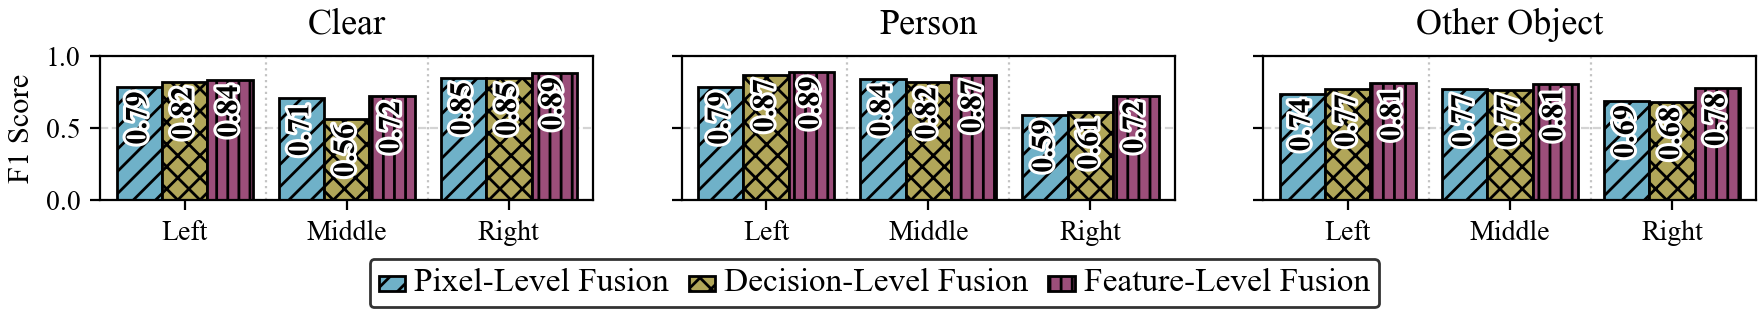
\includegraphics[width=\textwidth]{figs/fig2.png}
  \caption{Per-class $F_1$ by camera direction (left, middle, right) for the
  three fusion strategies: pixel (stitched), decision
  (output fusion), and feature.}
  \label{fig:arch_f1}
\end{figure*}

We evaluate four architectures for estimating per-direction navigability
from three ultra-low-resolution thermal cameras. All models operate directly
on raw single-channel $32\times24$ thermal tiles and produce a three-class
prediction (\textit{clear}, \textit{person}, or \textit{other object}) for
each camera direction. The architectures differ only in how information from
the three views is combined, spanning pixel-level, decision-level, and
feature-level fusion, together with a fourth variant that augments
feature-level fusion with camera-identity correction for placement
robustness. 
Except for the stitched-panorama baseline, all models share the same
convolutional backbone. The backbone consists of a stack of convolutional
blocks whose depth, width multiplier, and activation function are varied
during model selection. Each backbone produces multi-scale feature maps that
are consumed by the downstream fusion and classification modules.
% Except for the stitched-panorama baseline, all models share the
% same convolutional backbone.


% We evaluate four architectures for estimating per-direction navigability from the three active thermal cameras (left, middle, right), each consuming only raw $32\times24$ thermal tiles at inference time and producing a 3-class prediction per camera over $\{\text{clear}, \text{person}, \text{other object}\}$. Tiles are kept as single-channel raw intensity throughout, with no colorization step converting them to pseudo-RGB before the backbone, unlike prior work that colorizes thermal frames for a detector pretrained on natural images. The four span pixel-level, decision-level, and feature-level fusion, plus a fourth variant that adds a learned correction for camera-placement permutations on top of feature-level fusion. All but the stitched-panorama baseline share one configurable convolutional backbone, referred to below as the \textit{shared backbone}. This backbone is a plain stack of convolutional blocks with tunable depth $d \in \{2,\dots,5\}$, a MobileNets-style width multiplier $w$ that scales the channel count of every layer~\cite{howardMobileNetsEfficientConvolutional2017}, and a choice of activation $a \in \{\text{ReLU}, \text{GELU}, \text{LeakyReLU}\}$. It returns the intermediate feature map at every block so that downstream heads can pool over multiple resolutions.

\paragraph{Model 1: Stitched Panorama (pixel-level fusion)}
The three thermal tiles are first warped into a shared panoramic image using
pre-computed thermal-to-thermal homographies, following prior homography-based
thermal alignment approaches~\cite{dahmaniThermalHomographyPhotovoltaic2025,ansarPerformanceEvaluationFeature2024}. A convolutional backbone then predicts
the navigability state of each camera direction from the stitched panorama.
Because fusion occurs before feature extraction, information lost during the
homography warp cannot be recovered by subsequent layers.

% \paragraph{Model 1: Stitched Panorama (pixel-level fusion)} The three raw tiles are warped into a shared panoramic canvas via pre-computed thermal-to-thermal homographies, following prior homography-based approaches to close-range thermal alignment~\cite{dahmaniThermalHomographyPhotovoltaic2025,ansarPerformanceEvaluationFeature2024}. Nearest-neighbor interpolation ensures that warped pixels retain their original raw thermal values rather than being blended with neighbors or with the zero-padded border, yielding a two-channel panorama (raw intensity plus a validity mask). A fixed five-layer backbone is applied independently to each camera's bounding-box crop of the panorama, followed by a shared classification head. Because the panorama is built once, before any learned processing, cross-camera information lost to the homography warp is unavailable to the model. This baseline therefore isolates the cost of fusing at the pixel level.

\paragraph{Model 2: Output Fusion (decision-level fusion)} The shared backbone processes each camera's tile independently, and a per-camera head reduces it to one 3-class logit vector. The three logit vectors are concatenated and passed through a small fusion MLP that refines them jointly. Fusion only ever sees already-classified, low-dimensional logits, so cross-camera interaction is limited to statistical dependencies between directions rather than raw spatial features.
\paragraph{Model 3: Feature Fusion} The same shared-weight backbone runs on each camera's tile, but instead of classifying each camera separately, the feature maps from all three cameras at a given backbone level are concatenated channel-wise and projected back to the original channel count via a learned $1\times1$ convolution, applied at every level. This yields a single fused multi-scale feature pyramid mixing all three cameras at every depth, in contrast to Model 2's late fusion. A shared head then produces the final per-camera logits. We sweep backbone depth, width, activation, and head capacity to select the configuration used as the reference Feature Fusion result throughout this paper. The best-performing configuration uses a backbone depth of 5, a width multiplier of $1.5\times$, GELU activation, a 512-unit classification head, and a dropout rate of $0.1$, and this is the configuration used for Models 3 and Model 4 throughout the rest of the paper.


\paragraph{Model 4: Feature Fusion with camera-identity correction}
Feature Fusion assumes a fixed correspondence between input channels and
physical camera directions, making it sensitive to changes in camera
arrangement. To improve deployment robustness, we introduce a lightweight
camera-identity classifier that predicts the physical direction
(\textit{left}, \textit{middle}, or \textit{right}) of each thermal tile.
Given a possibly shuffled set of tiles, the classifier selects the most likely
camera-to-direction assignment, and the re-ordered tiles are passed to the
unmodified Feature Fusion model. We compare this approach against a blind
condition with no correction and an oracle condition using ground-truth camera
identities.


% \paragraph{Model 4: Feature Fusion with camera-identity correction} Model 3's per-level $1\times1$ projections consume all cameras' features in a fixed slot order, so the projection layer can learn to associate an input slot with a physical direction even though the backbone itself is fully shared and permutation-agnostic. If a sensor is reattached in a different slot at deployment time, this learned positional dependence can degrade predictions. We correct for it with a lightweight auxiliary camera-identity classifier, a compact CNN separate from the shared backbone that takes one raw thermal tile and predicts a 3-way softmax over $\{\text{left}, \text{middle}, \text{right}\}$. The classifier is trained independently using the true camera-to-direction mapping recorded at capture time (its slot-identification accuracy is reported in Section~\ref{sec:results}). At inference, given a possibly shuffled set of tiles, it scores every slot against every direction and selects the assignment that maximizes the total log-probability, enumerated exhaustively over all $3! = 6$ permutations. The re-sorted tiles are then passed to the unmodified Model 3. We compare this against an oracle re-sort using ground-truth identities (an upper bound on achievable robustness) and a blind condition with no correction at all.

All four architectures share the same masked, per-camera, three-class cross-entropy training objective, gated by a per-camera validity mask so that timesteps without a labeled RGB frame do not contribute gradient.
